\documentclass[a4paper,12pt]{article}
\usepackage{ctex} 
\usepackage{amsmath}
\usepackage{amsfonts}
\usepackage{graphicx}
\usepackage{tabularx}
\usepackage{caption}
\usepackage{subcaption}
\usepackage{geometry}
\usepackage{booktabs}
\usepackage{enumitem}
\usepackage{hyperref}
\usepackage{float}  % 用于 H 浮动控制
\usepackage{subcaption}
\usepackage[titletoc,toc,title]{appendix}

\title{GPT-1 预训练语言模型阅读报告}
\author{丁竞 PB22030826 胡延伸 PB22050983}
\date{}

\begin{document}

\maketitle

\section*{合作分工说明}

本报告由 \textbf{丁竞(PB22030826)} 与 \textbf{胡延伸(PB22050983)} 共同完成,具体分工如下:

\begin{itemize}
    \item \textbf{丁竞} 主要负责模型结构部分撰写与理论分析,包括:
    \begin{itemize}
        \item GPT 架构详解(位置编码、多头注意力、Transformer Block 等);
        \item 学习率调度策略与数学公式推导;
        \item 方法局限与改进方向归纳;
        \item 附录中 Transformer 数学推导与 MLE 理论分析。
    \end{itemize}

    \item \textbf{胡延伸} 主要负责实验与任务设计部分撰写与分析,包括:
    \begin{itemize}
        \item 预训练语料 BooksCorpus 的优势分析;
        \item 各类下游任务的统一 token 流建模策略;
        \item 任务实验结果(MNLI、RACE、Story Cloze 等)解读;
        \item GPT 系列后续演进(GPT-2/3、InstructGPT、ChatGPT)整理。
    \end{itemize}

    \item 二人协同完成摘要撰写、图表复现、报告排版与结构组织,并共同阅读原论文,确保内容准确、表达清晰、逻辑完整。
\end{itemize}

\vspace{1em}


\begin{abstract}
    本文围绕 2018 年 OpenAI 提出的预训练语言模型 GPT-1(Generative Pre-Training Transformer)展开阅读与分析。该模型首次系统性地提出“无监督预训练 + 有监督微调”的统一框架,并在多种自然语言处理任务中取得了突破性成果。论文采用 Transformer decoder-only 架构,通过自回归语言建模在 BooksCorpus 数据集上进行预训练,随后以统一的 token 序列格式微调于文本分类、问答、自然语言推理等任务。实验显示,GPT-1 在包括 MNLI、RACE、Story Cloze 等数据集在内的多个任务上显著优于此前方法,展现出强大的泛化能力与迁移性能。本文详细解析了模型的架构、训练目标函数、学习率调度策略、位置编码方式、多头注意力参数构成,并结合实际图表与数学推导对 GPT 的创新点进行了深入总结。同时,报告也指出了该方法的局限性,并从结构、目标函数与训练效率三个角度探讨了未来改进方向。
    \end{abstract}
    

    \section{NLP预训练技术的发展与GPT的突破}

    \subsection{从词向量到上下文建模:预训练的发展脉络}
    
    在机器学习中,\textbf{预训练}是指在无任务特定偏好的大规模语料上,通过自监督或弱监督信号训练模型,以学习通用语言表征,从而提升下游任务的泛化能力。自然语言处理领域的预训练技术发展经历了从静态词向量到上下文建模、再到统一语言模型范式的演进过程,如图所示:
    
    \begin{figure}[H]
        \centering
        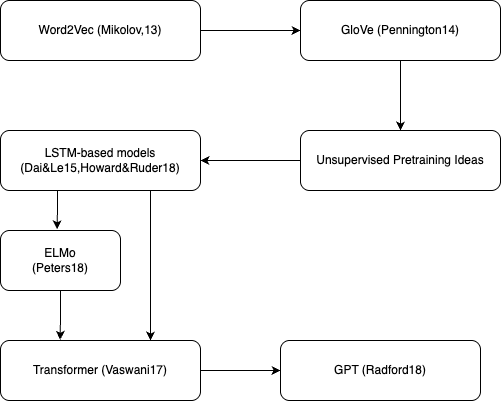
\includegraphics[width=0.8\textwidth]{image/发展脉络.png}
        \caption{预训练语言模型的发展路径}
    \end{figure}
    
    \paragraph{Word2Vec:静态词嵌入}
    
    在预训练尚未流行的早期阶段,NLP 任务通常依赖监督学习和手工设计特征。Word2Vec 是首批将无监督学习引入词向量建模的工作之一,提出 CBOW 与 Skip-gram 两种训练方式,通过上下文预测学习词的分布式表示。虽然能捕捉词义相似性,但其生成的词向量是静态的,难以处理多义词或语境变化。
    
    \paragraph{ELMo:上下文感知的动态词向量}
    
    ELMo 则引入了双向语言模型,生成根据上下文动态变化的词向量。该方法在预训练阶段构建 forward 和 backward 的 LSTM 语言模型,并将多层隐藏状态进行加权融合,显著提升了词表示对语法与语义的建模能力。ELMo 的成果奠定了语言模型用于下游迁移的实践基础。
    
    \subsection{GPT的提出与创新}
    
    尽管 ELMo 和 ULMFiT 等模型开启了语言模型预训练的方向,但其迁移仍受限于特征提取或结构改动。GPT 系列首次将 Transformer 架构与语言建模任务结合,采用 decoder-only 模型结构,从左至右地建模 token 序列:
    
    \begin{itemize}
        \item 使用标准语言模型作为预训练目标(预测下一个 token);
        \item 模型结构为纯 Transformer Decoder,无需特殊任务模块;
        \item 所有下游任务统一表示为文本生成问题,实现少量甚至零样本迁移;
        \item 通过微调机制,显著提升多项 NLP 任务的性能,展现强泛化能力。
    \end{itemize}
    
    GPT 相比同期方法的主要差异见表 \ref{tab:pretrained_models_comparison}:
    
    \begin{table}[H]
        \centering
        \begin{tabularx}{\textwidth}{|l|X|X|X|X|}
            \hline
            \textbf{维度} & \textbf{GPT} & \textbf{BERT} & \textbf{ELMo} & \textbf{ULMFiT} \\
            \hline
            \textbf{主干结构} & Transformer 解码器 & Transformer 编码器 & 双向 LSTM & 单向 LSTM \\
            \hline
            \textbf{输入} & 单向 token 序列 & 双向句子对 & 句子 & 句子 \\
            \hline
            \textbf{预训练目标} & 语言模型(左到右) & Masked LM、NSP & 前向 + 后向语言模型 & 语言模型 \\
            \hline
            \textbf{任务适配} & 拼接为 token 流统一建模 & 任务输入需 segment 标注 & 提供词向量特征 & 任务微调 \\
            \hline
            \textbf{迁移方式} & 微调 & 微调 & 特征提取 & 微调 \\
            \hline
            \textbf{代表优势} & 简单通用,适合生成任务 & 理解能力强,适合句对推理 & 融合上下文特征表达 & 易训练,适配多任务 \\
            \hline
        \end{tabularx}
        \caption{GPT、BERT、ELMo、ULMFiT 模型比较}
        \label{tab:pretrained_models_comparison}
    \end{table}
    
    \subsection{GPT在2018年的技术突破点}
    
    GPT 的提出标志着 NLP 预训练进入“统一语言建模框架”时代,主要贡献如下:
    
    \begin{enumerate}
        \item \textbf{统一训练范式}:首次提出预训练 + 微调的通用策略,一个模型结构可适配多种任务,减少了任务特定改动与特征设计需求;
        \item \textbf{引入 Transformer 结构}:相比 RNN/LSTM 更适合长依赖建模,且无需重设计网络即可迁移到下游任务;
        \item \textbf{语言建模直接迁移}:利用无监督训练目标,在多个任务上通过简单微调即可超越传统监督方法,刷新 9 项 NLP 基准任务;
        \item \textbf{奠定大型语言模型范式}:开启了后续 GPT-2、GPT-3、InstructGPT 乃至 ChatGPT 等大模型的发展路线,影响深远。
    \end{enumerate}
    

\section{模型架构}

\subsection{预训练语料 BooksCorpus 的选择与优势}

GPT-1 的预训练采用了 BooksCorpus 数据集,这是一份由 11,038 本未出版英文小说组成的语料库,总文本规模约为 7,000 万句、近 8 亿词(tokens)。这些文本以连续段落的形式呈现,具有较强的上下文连贯性和长程语义依赖结构。

与传统语料如 1B Word Benchmark 相比,BooksCorpus 拥有显著优势:

\begin{itemize}
    \item \textbf{长文本结构}:每本小说均保持原始章节和段落顺序,保留了自然语言中的长距离依赖,适合训练具备上下文理解能力的自回归模型。
    \item \textbf{未打乱顺序}:1B Word Benchmark 将句子顺序完全打乱,导致模型难以捕捉跨句上下文;而 BooksCorpus 维持原始文档结构,更贴合语言建模任务的真实场景。
    \item \textbf{语体一致、主题丰富}:小说文本多为叙述性文体,涵盖广泛话题,包括对话、描写、心理活动等,有利于模型学习多样化语言风格。
    \item \textbf{篇幅长、分布自然}:每本小说平均包含上万句文本,单个文档平均 token 长度远大于维基百科段落,有助于训练捕捉长程语义。
\end{itemize}

论文指出,选择 BooksCorpus 的一个重要考虑是其“具有长文档上下文结构”,这对于以语言建模作为训练目标的 GPT 来说至关重要。相比 Wikipedia,后者更适合用于 masked language modeling,而 BooksCorpus 更适合用于自回归预训练,符合 GPT 架构和训练方式的需求。


\subsection{位置编码}

Transformer 论文中首次提出“位置编码”,让模型感知输入序列中各token的位置信息,解决自注意力结构对顺序不敏感的问题。

主要有两种实现方式:

\begin{enumerate}
    \item 正弦/余弦(Sinusoidal):用确定性函数编码每个位置。
    \item 学习式(Learned):把每个位置作为索引,直接训练一个可学习的embedding表。
\end{enumerate}


而 GPT 论文明确指出:“我们使用learned position embeddings,而不是原始Transformer中的sinusoidal编码。”(原文:“We used learned position embeddings instead of the sinusoidal version proposed in the original work.”)

论文进行了实验,得到如下结论:


\begin{table}[H]
    \centering
    \begin{tabularx}{\textwidth}{|l|X|X|X|}
        \hline
        \textbf{方式} & \textbf{原理} & \textbf{特点} & \textbf{GPT实验结论} \\
        \hline
        \textbf{正弦式} & 位置通过公式 $PE(pos,2i)=\sin(pos/10000^{2i/d})$ 等,固定不可训练 & 不易过拟合,对长文本泛化好,天然支持外推到未见过的位置 & 无GPT直接实验对比,但原始Transformer证明有效,实际工程中对超长文本略有优势 \\
        \hline
        \textbf{学习式} & 位置embedding可与token embedding类似,训练中不断优化 & 更灵活,可感知特定任务中的位置信号,容易拟合训练分布,但对极长句泛化略差 & GPT采用此方式,训练效果优良,短-中长度任务表现更优 \\
        \hline
    \end{tabularx}
    \caption{位置编码方式的对比}
    \label{tab:positional_encoding_comparison}
\end{table}

\subsection{激活函数与归一化策略}

GPT-1 中的每层 Transformer 使用 \textbf{GELU(Gaussian Error Linear Unit)} 激活函数代替传统的 ReLU,其定义如下:
\[
\text{GELU}(x) = x \cdot \Phi(x), \quad \Phi(x) = \frac{1}{2} \left[1 + \text{erf}\left(\frac{x}{\sqrt{2}}\right)\right]
\]

相比于 ReLU,GELU 提供更平滑的非线性变换,提升了语言建模任务中模型的拟合能力和泛化性能。

同时,全模型广泛使用 \textbf{Layer Normalization},在注意力层与前馈网络之后分别添加,缓解深层网络中的梯度爆炸与收敛不稳定问题。

\subsection{残差连接的作用}

每个子层(如 Attention、FFN)后均配有残差连接(Residual Connection):
\[
\text{Output} = \text{LayerNorm}(x + \text{SubLayer}(x))
\]

这种设计灵感来源于图像领域的 ResNet,允许梯度直接穿过多个层,有效缓解了深度网络训练中的退化问题,保证了 12 层深度 Transformer 的可训练性与稳定性。



\subsection{多层 Transformer Decoder 的结构简析}

GPT-1 的模型采用了标准的 Transformer Decoder-only 堆叠结构,共包含 12 层、每层 12 个注意力头、每头维度为 64,总 hidden size 为 768。输入经过 token embedding 与位置嵌入相加后,依次通过 masked multi-head self-attention、前馈网络和残差连接。输出经过共享的词向量矩阵映射至词表,完成下一 token 的预测。

如图\ref{fig:transformer_decoder_structure}所示,GPT 的 Transformer Decoder 结构主要由以下几个部分组成:
\begin{itemize}
    \item \textbf{输入嵌入(Input Embedding)}:将输入 token 转换为向量表示,并添加位置编码。
    \item \textbf{Masked Multi-Head Self-Attention}:每层使用多头自注意力机制,允许模型关注输入序列中不同位置的信息。注意力机制通过掩码确保每个 token 只能看到其左侧的上下文。
    \item \textbf{前馈网络(Feed-Forward Network)}:每层包含一个前馈神经网络,通常由两个线性变换和一个非线性激活函数(如 GELU)组成。
    \item \textbf{残差连接与层归一化(Residual Connection and Layer Normalization)}:每个子层后都有残差连接和层归一化,以帮助梯度流动和稳定训练。
    \item \textbf{输出预测(Output Prediction)}:最后一层的输出通过一个线性变换映射到词表大小的向量,使用 softmax 计算每个 token 的概率分布。
\end{itemize}

\begin{figure}[H]
    \centering
    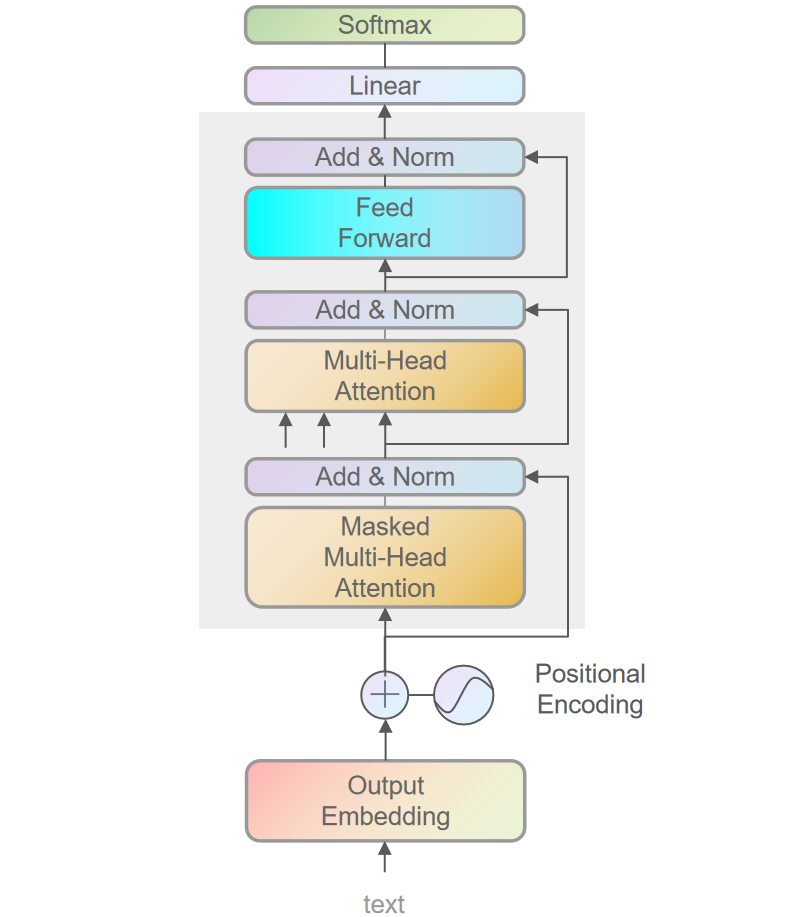
\includegraphics[width=0.5\textwidth]{image/image1.png}
    \caption{GPT-1 的 Transformer Decoder 结构}
    \label{fig:transformer_decoder_structure}
\end{figure}

该结构的数学细节可参考本文附录 \ref{appendix:transformer_math},包含了完整的注意力计算、前馈过程与预测公式推导。


\subsection{多头注意力参数}

多头自注意力机制允许模型从不同子空间捕捉多样化的特征关系。如图\ref{fig:multihead_attention}所示,GPT-1 的多头注意力机制将输入向量 $X$ 通过三个线性变换得到查询(Q)、键(K)和值(V)矩阵,然后计算每个头的注意力输出,最后将所有头的输出拼接并通过线性变换得到最终结果:

\begin{figure}[H]
    \centering
    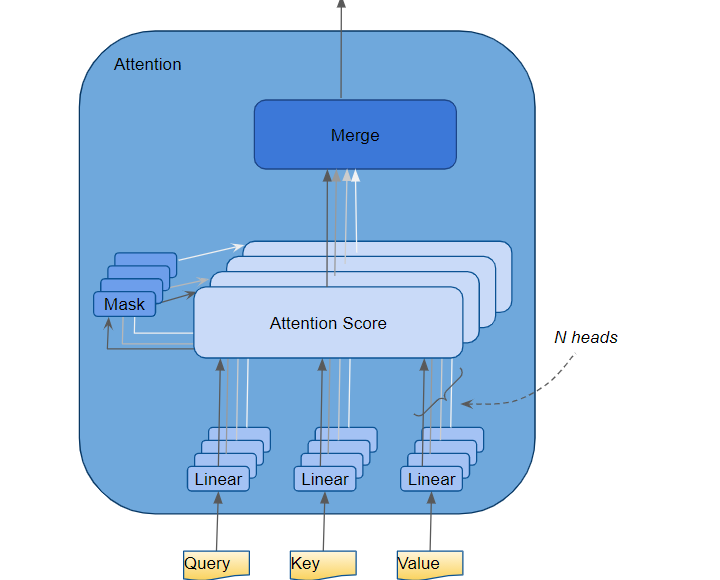
\includegraphics[width=0.8\textwidth]{image/多头注意力.png}
    \caption{多头注意力机制示意图}
    \label{fig:multihead_attention}
\end{figure}

“头数”直接影响:1)模型参数量;2)模型表达能力;3)并行计算速度。GPT用的是12层、12头注意力,每层hidden size为768。单层参数量近似分布如下(略去偏置/小项,仅主结构):

\begin{table}[H]
    \centering
    \begin{tabularx}{\textwidth}{|l|X|X|X|}
        \hline
        \textbf{组件} & \textbf{参数公式} & \textbf{以12头为例} & \textbf{其他配置(如6/24头)影响} \\
        \hline
        Q/K/V投影 & $3 \times d_\text{model} \times d_\text{model}$ & $3 \times 768 \times 768$ & 头数不影响总参数,只影响每头维度 \\
        \hline
        多头输出 & $d_\text{model} \times d_\text{model}$ & $768 \times 768$ & 同上 \\
        \hline
        \textbf{总和} & $\approx 4 \times d_\text{model} \times d_\text{model}$ & $\approx 2.36$M/层 & 基本不变 \\
        \hline
    \end{tabularx}
    \caption{多头注意力层参数量分析}
    \label{tab:multihead_attention_params}
\end{table}

\textbf{头数改变对参数占比/模型影响}

\begin{itemize}
    \item 增减“头数”不会改变总参数量(hidden size保持不变),但会调整每头的维度(如12头时每头64维,6头时每头128维)。
    \item 多头的优势在于捕获不同特征;但头太多会导致每头的信息量变少、表达稀疏;头太少会减少表达多样性。
    \item 实验上(见BERT、GPT等),12头是综合效果和硬件效率的平衡。
\end{itemize}


GPT论文未专门消融“头数”,但选用12头原因:

\begin{itemize}
    \item 768维hidden size下分12头,每头64维,既有丰富信息又便于并行(GPU友好)。
    \item 后续GPT-2(hidden size=1600, heads=25)、GPT-3(hidden size=12288, heads=96),头数均随hidden size增大等比例扩展。
\end{itemize}

Transformer原始论文也给出了类似建议:“头数越多,感知的子空间越多,但每头信息量变稀释,过少过多都会有副作用。”

\subsection{模型参数总量与计算复杂度}

GPT-1 模型包含约 \textbf{117M 参数},主要集中在:

\begin{itemize}
    \item 词嵌入矩阵 $W_e \in \mathbb{R}^{V \times d}$,词表大小 $V = 40,000$,嵌入维度 $d=768$;
    \item 每层 Transformer 模块中的 Attention 与 FFN 层;
    \item 总体参数量与 GPT-2(1.5B)相比低 1 个数量级,便于实验室规模复现。
\end{itemize}

尽管参数相对较少,但 Transformer 每层 Attention 的计算复杂度为 $\mathcal{O}(n^2 d)$,其中 $n$ 为输入 token 序列长度,因此推理时仍需注意内存与算力配置。

\subsection{小结}

综上所述,GPT-1 架构在当时的创新体现在:

\begin{itemize}
    \item 首次大规模使用 Transformer Decoder-only 模型进行自回归语言建模;
    \item 精选 BooksCorpus 长文本语料训练,优化上下文建模能力;
    \item 灵活采用可学习位置编码、多头注意力与 GELU 激活,提升训练效率与泛化性能;
    \item 构建了统一输入、统一输出、统一架构的预训练语言建模框架,极大简化了下游任务适配难度。
\end{itemize}


\section{训练策略与任务统一格式设计}

GPT 模型采用无监督的语言建模预训练目标,即最大化 token 序列中每个词在其左侧上下文条件下的概率。这种自回归方式使得模型天然适用于生成类任务,同时也为后续的统一任务建模奠定基础。

\subsection{语言建模目标函数简析}

在预训练阶段,模型输入一段 token 序列 $U = \{u_1, u_2, \dots, u_k\}$,训练目标是最大化当前 token 在其历史上下文条件下出现的概率,即最大化如下对数似然:

\[
\mathcal{L}_{\text{pretrain}}(U) = \sum_{i=1}^{k} \log P(u_i \mid u_{<i})
\]

这一过程本质上是最大似然估计(MLE)框架的具体实例,关于其理论收敛性与优化性,可参考附录 \ref{appendix:mle_proof}。

\subsection{任务统一:Token流视角的建模策略}

为了让同一个预训练模型能适配多种下游任务,GPT 将各类任务统一转化为纯文本的 token 序列,从而以语言建模的方式进行微调。该设计避免了任务特定的架构改动,体现了极强的迁移通用性。

\begin{table}[H]
    \centering
    \caption{不同任务如何转化为统一 token 序列进行微调}
    \label{tab:task_unification}
    \begin{tabularx}{\textwidth}{|l|X|X|}
        \hline
        \textbf{任务类型} & \textbf{输入转换方式} & \textbf{目标预测位置} \\
        \hline
        文本分类(SST-2) & 将句子原文拼接上标签提示词(如“Positive or Negative?”) & 预测标签 token \\
        \hline
        自然语言推理(MNLI) & 拼接前提和假设,如“Premise: ... Hypothesis: ...” & 预测“entailment / contradiction / neutral” \\
        \hline
        问答(RACE) & 拼接问题 + 选项 + 文章内容 & 预测正确答案选项(A/B/C/D) \\
        \hline
        常识推理(Story Cloze) & 拼接故事前文和候选结局句 & 预测最合适结局句子 \\
        \hline
        语义相似度(QQP) & 拼接两个句子 + 提示短语(如“Are they duplicates?”) & 预测“yes / no” \\
        \hline
    \end{tabularx}
\end{table}

\begin{figure}[H]
    \begin{subfigure}[b]{0.5\textwidth}
        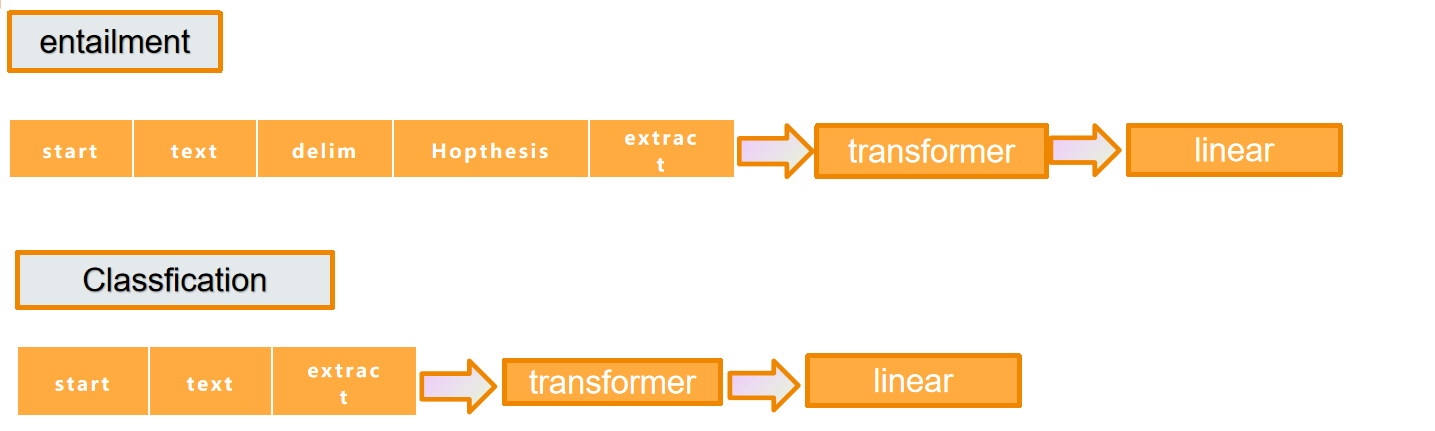
\includegraphics[width=\textwidth]{image/image2.png}
        \caption{}
    \end{subfigure}
    \hfill
    \begin{subfigure}[b]{0.5\textwidth}
        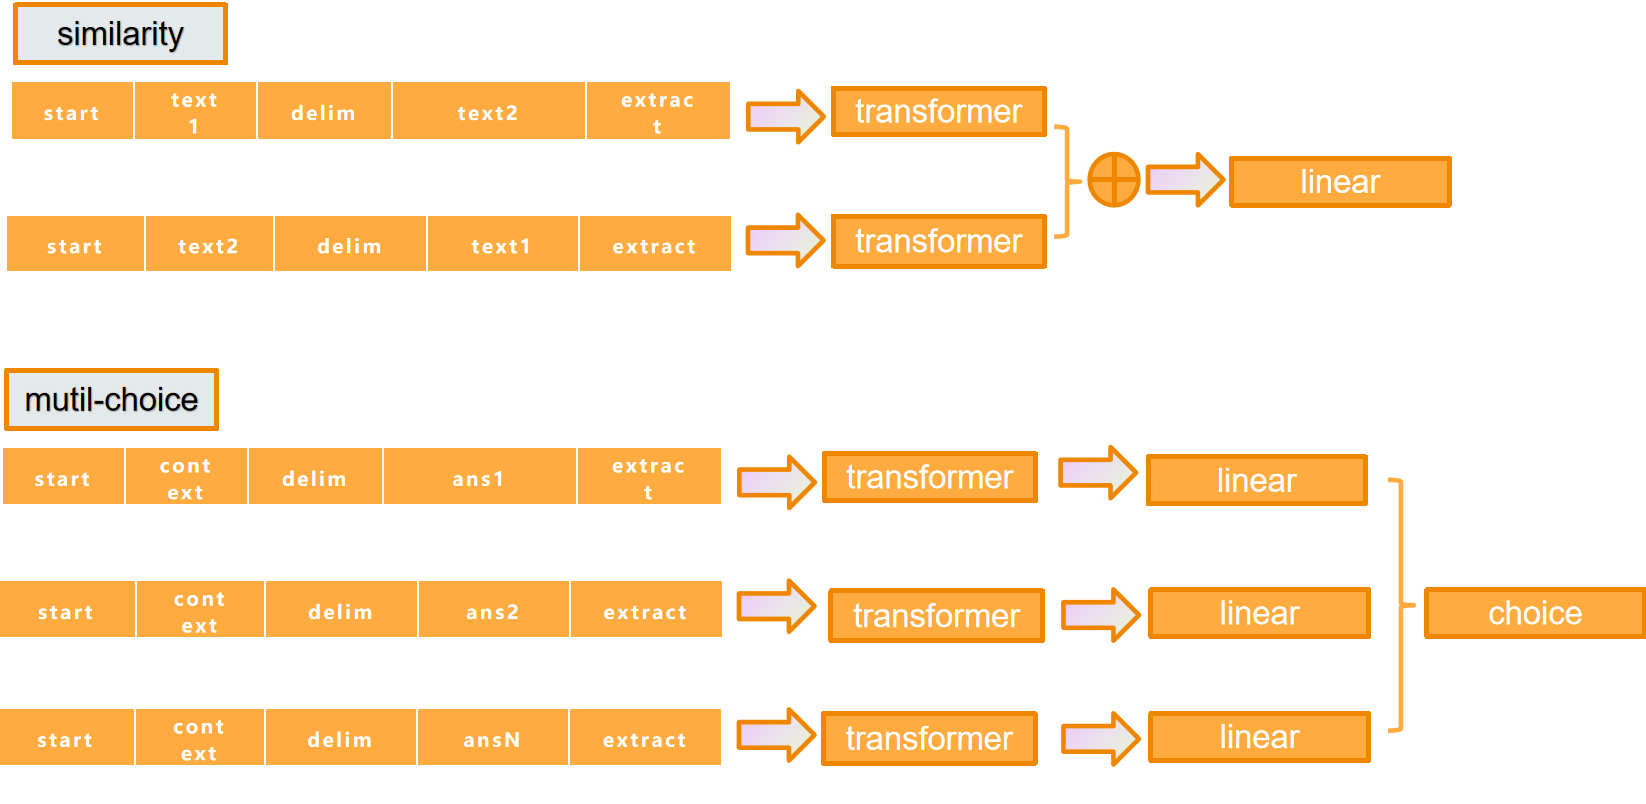
\includegraphics[width=\textwidth]{image/image3.png}
        \caption{}
    \end{subfigure}
    \caption{任务统一的 token 流示图}
\end{figure}

这种方式使得 GPT 能够在统一的训练机制下,同时适配分类、生成、排序等任务,避免了多任务模型架构切换的成本,也说明了其“统一语言模型”范式的优势。


\subsection{GPT 学习率预热曲线}

根据论文(Radford et al., 2018)中描述的学习率策略:

% * 
% * 
% * **最大学习率**:`2.5e-4`
% * **预热步数**:`2000 steps`
% *
% * 

\begin{itemize}
    \item \textbf{优化器}:Adam
    \item \textbf{初始学习率}:0(从0开始预热)
    \item \textbf{预热步数}:2000 steps
    \item \textbf{整体调度}:线性预热 + Cosine Decay
    \item \textbf{总训练步数}:约 100 epochs,每 epoch ≈ minibatch of 64 sequences of 512 tokens(总训练步数可根据实际设置)
\end{itemize}

因此大致可推导出如下学习率调度公式:

$$
lr(step) = 
\begin{cases}
\text{linearly increase from 0 to } lr_{\text{max}}, & step \leq 2000 \\
lr_{\text{max}} \times 0.5 \times (1 + \cos(\frac{\pi \times (step - 2000)}{T - 2000})), & step > 2000
\end{cases}
$$

得到曲线如下图所示:

\begin{figure}[H]
    \centering
    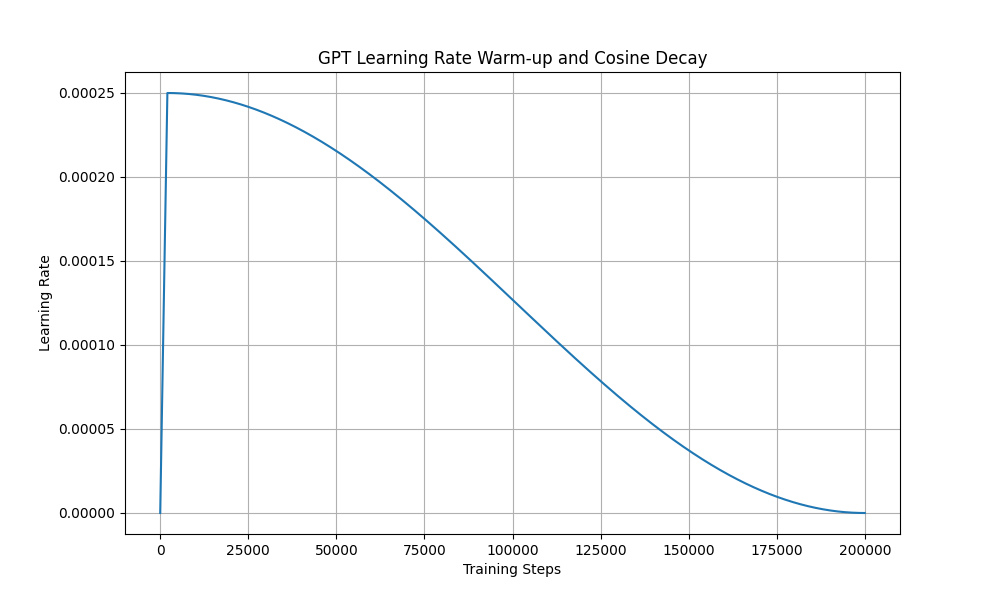
\includegraphics[width=0.8\textwidth]{image/Figure_1.png}
    \caption{GPT学习率预热曲线}
\end{figure}

\section{实验结果与分析}

\begin{figure}[h]
    \centering
    \begin{subfigure}[b]{0.45\textwidth}
        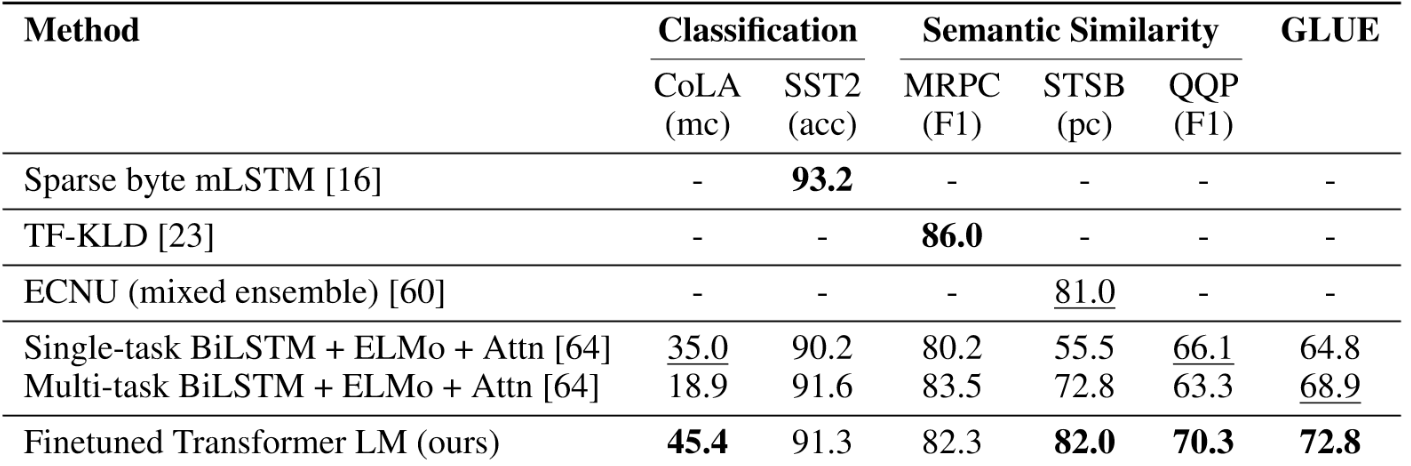
\includegraphics[width=\textwidth]{image/image7.png}
        \caption{}
    \end{subfigure}
    \hfill
    \begin{subfigure}[b]{0.45\textwidth}
        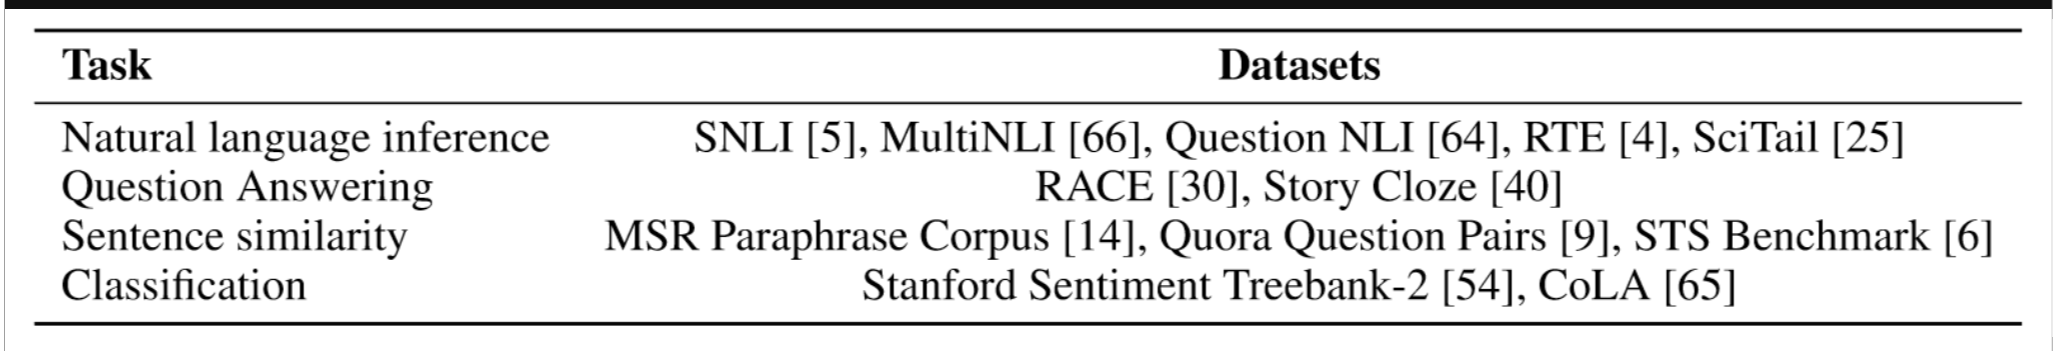
\includegraphics[width=\textwidth]{image/image4.png}
        \caption{}
    \end{subfigure}
    \vskip\baselineskip
    \begin{subfigure}[b]{0.45\textwidth}
        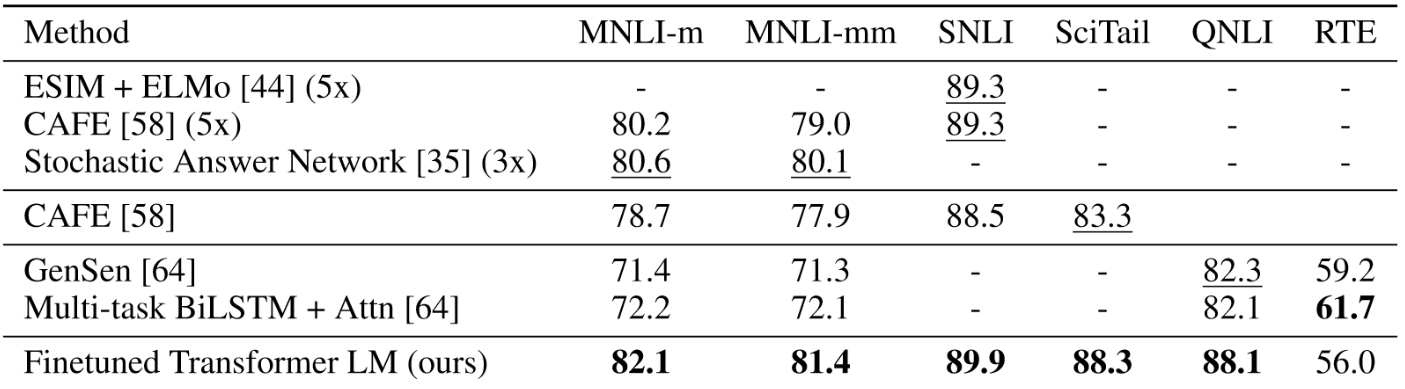
\includegraphics[width=\textwidth]{image/image5.png}
        \caption{}
    \end{subfigure}
    \hfill
    \begin{subfigure}[b]{0.45\textwidth}
        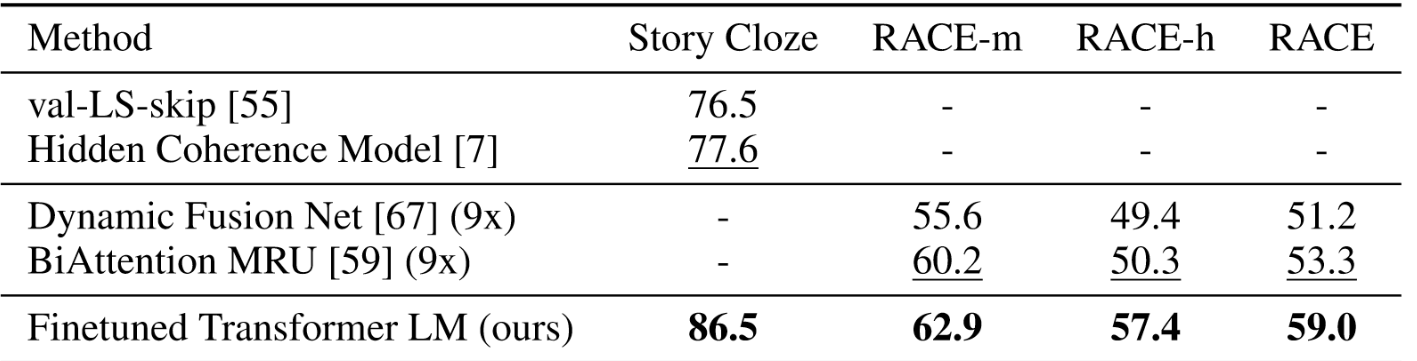
\includegraphics[width=\textwidth]{image/image6.png}
        \caption{}
    \end{subfigure}
    \caption{实验结果图}
\end{figure}

\subsection{自然语言推理}

GPT 模型在自然语言推理任务中展现出显著的迁移能力。在 \textbf{MultiNLI} 任务中,模型达到了 \textbf{82.1\%} 的准确率,相比先前最优模型提升了 \textbf{3.8\%}。在 \textbf{QNLI} 数据集上,准确率提升至 \textbf{88.1\%},在 \textbf{SciTail} 数据集上达到 \textbf{88.3\%},整体性能超过了传统基于双向 LSTM 或 BiDAF 架构的方法。这些结果表明,通过语言建模方式预训练的 GPT 架构,能够捕获丰富的上下文语义与逻辑信息,有效迁移到句对推理任务。

\subsection{问答与常识推理}

在问答类任务中,GPT 在 Story Cloze Test 上实现了 \textbf{86.5\%} 的准确率,相较于传统方法提升了 \textbf{8.9\%}。在 \textbf{RACE} 阅读理解任务上,整体准确率达到 \textbf{59.0\%},提升幅度超过 \textbf{5\%}。这类任务通常需要模型具备跨句推理能力和一定的常识推断能力,GPT 在预训练过程中通过学习长篇连续文本的语言结构,显著增强了这类能力,体现了生成式语言建模在非生成任务中的迁移价值。

\subsection{语义相似度与分类任务}

在语义匹配与句子分类任务中,GPT 同样展现出出色表现。在 \textbf{STS-B} 任务中,Pearson 相关系数达到 \textbf{82.0},远高于前最佳模型的 \textbf{75.5};在 \textbf{QQP} 任务中 F1 分数为 \textbf{70.3\%},较前一最佳结果提高约 \textbf{4.2} 个百分点。分类任务方面,模型在 \textbf{CoLA} 上达到了 \textbf{45.4} 的 Matthew's correlation,超过先前 SOTA(35.0);在情感分类数据集 \textbf{SST-2} 上,准确率为 \textbf{91.3\%}。这些结果证明了预训练语言模型在句子层级语义理解与结构敏感性任务中的强大迁移能力。

\subsection{综合GLUE得分分析}

GPT 在 GLUE 多任务评估框架中整体得分达到 \textbf{72.8},相较于此前最佳方法的 \textbf{68.9} 有显著提升,且在 \textbf{12 个任务中有 9 项刷新了 SOTA}。特别值得注意的是,GPT 无需为每个任务设计独立模型结构,仅通过统一的 token 流输入与微调即可实现泛化迁移,这种高度的统一性和通用性为后续大模型预训练范式奠定了基础。

此外,作者进一步分析了预训练深度对下游任务的迁移效果,发现 Transformer 每一层都学习到了可迁移知识,随着模型深度增加,任务性能逐步提升。这一发现支持了“深层语言模型 = 多级语义编码器”的观点,也解释了为何大规模预训练在多个任务中均能有效迁移。




\section{方法局限与理论改进}

\subsection{现有方法的不足}

虽然 GPT-1 在多个任务上取得了显著性能提升,但其方法本身仍存在诸多限制:

\begin{table}[H]
    \centering
    \caption{GPT-1 方法的不足}
    \begin{tabular}{|p{4cm}|p{8cm}|}
        \hline
        \textbf{缺陷} & \textbf{具体表现} \\
        \hline
        并行效率低 & 自回归架构限制并行性,特别是在推理时无法同时预测多个 token \\
        计算复杂度高 & 长序列 + 全局 self-attention,导致注意力计算成本为 $O(n^2)$ \\
        单向建模 & 只能利用历史上下文,无法整合未来信息,限制语义建模能力 \\
        训练资源开销大 & 依赖小 batch 和多 epoch 训练,整体收敛速度慢,资源消耗高 \\
        词表设计限制 & 使用 BPE 分词策略,虽然高效但在处理多语言或稀有词汇时存在表达瓶颈 \\
        \hline
    \end{tabular}
\end{table}

\subsection{结构性改进(Architecture-Level Improvements)}

\subsubsection{双向建模(Bidirectional Modeling)}

传统的自回归语言模型仅利用前向上下文,限制了对全局语义的建模能力。BERT采用Masked LM实现双向建模,显著提升了理解类任务性能。进一步工作如XLNet通过置换语言建模(permutation-based LM)整合双向信息与自回归优势,表明混合方向性建模具有潜力。

\subsubsection{稀疏注意力(Sparse Attention)}

Transformer中全连接注意力机制的计算复杂度为$O(n^2)$,在处理长文本时效率低下。Reformer、Longformer、BigBird等通过引入局部块、稀疏图结构或可学习注意力,显著降低复杂度。未来可探索结构对齐的稀疏模式(如基于句法依赖树)或内容感知注意力机制。

\subsection{预训练目标与学习方法改进}

\subsubsection{统一预训练目标(Unified Objectives)}

GPT-1仅采用下一个词预测(Next Token Prediction)作为训练目标,难以泛化到理解任务。BERT、T5等引入Masked LM、Span Prediction、Denoising等目标,从不同层面增强语义表示学习能力。未来可融合多种目标进行联合预训练,提升跨任务泛化性能。

\subsection{优化与训练效率提升(Efficiency-Oriented Enhancements)}

\subsubsection{优化器与调度策略}

早期训练采用Adam + Warmup + Cosine LR。为提升在大批量训练中的稳定性与效率,可引入自适应调度器(如LAMB、AdaFactor)或二阶优化方法(如Shampoo、K-FAC),从理论上改善收敛速度与泛化表现。

\subsubsection{参数压缩与低秩建模}

大规模语言模型存在显著冗余。方法如LoRA、模型蒸馏等基于低秩结构的压缩策略,显著降低计算开销。理论上可通过参数共享、子空间分解等方式构造轻量高效的表示空间。

\section{GPT-1 的影响与后续演进}

GPT-1 的提出不仅标志着预训练语言模型范式的转折点,也直接催生了一系列后续模型的发展,逐步推动了通用语言智能系统的形成。其“统一语言建模 + 微调”框架被验证为可扩展的基础,并在模型结构与训练规模上持续演进。

\subsection{GPT-2:扩大模型规模,推进纯生成方向}

GPT-2 延续 GPT-1 的 decoder-only 架构,但在规模上大幅扩展,参数量从 1.1 亿提升至 15 亿,训练语料也从 BooksCorpus 扩展为 40GB 的网络文本集合(WebText)。GPT-2 不再依赖任务特定微调,而是尝试将所有任务形式统一为“生成问题”,通过 few-shot / zero-shot 提示完成摘要、翻译、问答等任务。

主要创新点包括:

\begin{itemize}
    \item \textbf{大规模自回归语言建模}:验证语言模型参数规模对泛化能力的直接促进。
    \item \textbf{无监督泛化}:展示模型无需微调即可通过提示(prompt)完成任务。
    \item \textbf{安全争议}:出于滥用风险考虑,GPT-2 初期未完全开源,引发关于“开放”与“负责任 AI”之间的讨论。
\end{itemize}

\subsection{GPT-3:few-shot 能力的极限扩展}

GPT-3 进一步将参数规模扩展至 1750 亿,并采用更大的训练数据(570GB文本),几乎完全放弃下游微调,仅依靠 prompt 学习(in-context learning)在多项任务中达到甚至超过监督学习基线。

其核心突破包括:

\begin{itemize}
    \item \textbf{“任务即提示”}:通过自然语言提示学习任务结构,摆脱监督标签。
    \item \textbf{Few-shot 学习能力}:模型能从数个例子中学习新任务,表现出类人类的迁移与泛化行为。
    \item \textbf{通用性与风险并存}:模型展现出强大的语言生成能力,同时带来事实错误、幻觉等安全问题,引发对 AI 可控性的广泛关注。
\end{itemize}

\subsection{InstructGPT 与 ChatGPT:对齐优化与 RLHF 的引入}

面对 GPT-3 输出不准确、不符合用户意图等问题,OpenAI 提出了 InstructGPT 和 ChatGPT 系列,首次系统性引入 \textbf{强化学习人类反馈(RLHF)} 策略,让模型学会更“有用、诚实、无害”的对话能力。

主要改进如下:

\begin{itemize}
    \item \textbf{奖励模型(Reward Model)}:通过人工标注偏好数据训练奖励模型,引导模型输出更符合用户期待的响应。
    \item \textbf{策略微调(PPO)}:使用 Proximal Policy Optimization(PPO)等策略优化算法,在语言模型基础上进一步“强化学习”。
    \item \textbf{对话式优化}:ChatGPT 特别优化了多轮对话的连贯性、风格控制与用户意图识别能力,成为通用对话 AI 的典范。
\end{itemize}

这些改进体现了语言模型从“预测下一个 token”向“理解并回应人类意图”的过渡,也开辟了 AI alignment 的研究方向。



% 引入附录
\clearpage
\begin{appendices}
\renewcommand{\thesection}{A.\arabic{section}}

\section{Transformer Decoder 的数学推导}
\label{appendix:transformer_math}

\subsection{输入嵌入(Embedding + Position Encoding)}
输入 token 序列 $(u_1, \dots, u_k)$,经过嵌入层:
\[
h_0 = U W_e + P
\]
其中:
\begin{itemize}
    \item $U$ 是 token 的编码矩阵;
    \item $W_e \in \mathbb{R}^{V \times d}$ 为词嵌入矩阵;
    \item $P \in \mathbb{R}^{k \times d}$ 为位置嵌入矩阵。
\end{itemize}

\subsection{Transformer Block(第 $l$ 层)}

\paragraph{Masked Multi-Head Self-Attention}
每个注意力头 $i = 1, \dots, h$ 生成 Q/K/V:
\[
Q_i = H^{(l-1)} W_i^Q, \quad K_i = H^{(l-1)} W_i^K, \quad V_i = H^{(l-1)} W_i^V
\]
带掩码的注意力:
\[
\text{Attention}(Q_i, K_i, V_i) = \text{softmax}\left( \frac{Q_i K_i^\top}{\sqrt{d_k}} + M \right) V_i
\]
拼接所有注意力头:
\[
\text{MultiHead}(H^{(l-1)}) = \left[ \text{Attention}_1; \dots; \text{Attention}_h \right] W^O
\]
加残差连接与层归一化:
\[
\tilde{H}^{(l)} = \text{LayerNorm}\left( H^{(l-1)} + \text{MultiHead}(H^{(l-1)}) \right)
\]

\paragraph{前馈网络(Feed-Forward Network)}
\[
\text{FFN}(x) = W_2 \, \text{GELU}(W_1 x + b_1) + b_2
\]
\[
H^{(l)} = \text{LayerNorm}\left( \tilde{H}^{(l)} + \text{FFN}(\tilde{H}^{(l)}) \right)
\]

\subsection{输出预测}
最终输出 $H^{(L)}$ 投影到词表概率:
\[
P(u) = \text{softmax}\left( H^{(L)} W_e^\top \right)
\]
预测下一个 token 的条件概率:
\[
P(x_k \mid x_{<k}) = \text{softmax}\left( h_{k-1}^{(L)} W_e^\top \right)
\]

\section{最大似然估计的收敛性与优化性分析}
\label{appendix:mle_proof}

\subsection{最大似然估计的收敛性(Consistency of MLE)}

GPT 的训练目标属于最大似然估计(MLE)框架。给定参数化语言模型 $P_\theta$,其损失函数为:
\[
\mathcal{L}(\theta) = - \mathbb{E}_{U \sim P_{\text{true}}} \left[ \sum_{i=1}^{k} \log P_\theta(u_i \mid u_{<i}) \right]
\]

在满足以下条件时,MLE 是一致的(即 $\theta_n \xrightarrow{P} \theta^*$):
\begin{itemize}
    \item 参数空间 $\Theta$ 紧致;
    \item 对 $\theta$ 连续可导;
    \item 存在界函数 $g(U)$ 使得 $\log P_\theta(U) \leq g(U)$ 且 $g(U)$ 可积;
    \item 真分布 $P_{\text{true}} \in \{P_\theta\}$。
\end{itemize}

\subsection{训练过程的优化收敛性}

在实际训练中,我们优化的是经验风险:
\[
\hat{\mathcal{L}}(\theta) = - \frac{1}{n} \sum_{j=1}^{n} \sum_{i=1}^{k_j} \log P_\theta(u_i^{(j)} \mid u_{<i}^{(j)})
\]
使用如 Adam 的一阶优化器时,若满足:
\begin{itemize}
    \item 损失函数连续可微;
    \item 参数空间为欧氏空间 $\mathbb{R}^d$;
    \item 使用合适学习率调度(如 warm-up + decay);
\end{itemize}
则根据 Robbins-Monro 梯度下降理论,训练过程以概率收敛到局部最小值。
\end{appendices}

\end{document}